% main.tex

\documentclass[a4paper,12pt,oneside,openany,headsepline,bibliography=totocnumbered]{scrbook}

% Import settings, packages, etc.
% settings.tex

\newcommand{\thauthor}{Luis Falke}
\newcommand{\thtitle}{Side-Channel Resistant Implementations of Post-Quantum Cryptography}

\usepackage[T1]{fontenc}
\usepackage[utf8]{inputenc}
\usepackage{graphicx}
\usepackage{epstopdf}
\usepackage{amsmath}
\usepackage{amssymb}
\usepackage{amsfonts}
\usepackage{eucal}
\usepackage{fancyhdr}
\usepackage{url}
\usepackage{listings}
\usepackage[printonlyused]{acronym}
\usepackage{algorithmic}
\usepackage{algorithm}
\usepackage{multicol}
\usepackage{hyphenat}
\usepackage{cite}
\usepackage{subcaption}
\usepackage{etoolbox}

\makeatletter
\patchcmd{\chapter}{plain}{fancyplain}{}{}
\makeatother

% Custom styles for different sections
\fancypagestyle{chapterstart}{
    \fancyhf{}
    \fancyhead[L]{\slshape \leftmark}
    \fancyhead[R]{\thepage}
    \renewcommand{\headrulewidth}{0.4pt}
}

\fancypagestyle{abstract}{
    \fancyhf{}
    \fancyhead[L]{\slshape Abstract}
    \fancyhead[R]{\thepage}
    \renewcommand{\headrulewidth}{0.4pt}
}

\fancypagestyle{contents}{
    \fancyhf{}
    \fancyhead[L]{\slshape Table of Contents}
    \fancyhead[R]{\thepage}
    \renewcommand{\headrulewidth}{0.4pt}
}

\fancypagestyle{acronyms}{
    \fancyhf{}
    \fancyhead[L]{\slshape Acronyms}
    \fancyhead[R]{\thepage}
    \renewcommand{\headrulewidth}{0.4pt}
}

\fancypagestyle{listsoffigures}{
    \fancyhf{}
    \fancyhead[L]{\slshape List of Figures}
    \fancyhead[R]{\thepage}
    \renewcommand{\headrulewidth}{0.4pt}
}

\fancypagestyle{listoftables}{
    \fancyhf{}
    \fancyhead[L]{\slshape List of Tables}
    \fancyhead[R]{\thepage}
    \renewcommand{\headrulewidth}{0.4pt}
}

\fancypagestyle{bibliography}{
    \fancyhf{}
    \fancyhead[L]{\slshape Bibliography}
    \fancyhead[R]{\thepage}
    \renewcommand{\headrulewidth}{0.4pt}
}

% Graphics path
\graphicspath{{../figures/}}

% URL style
\urlstyle{tt}

% Separation between list items
\setlength{\itemsep}{0ex plus0.2ex}

% Fancy headers
\setlength{\headsep}{8mm}
\pagestyle{fancyplain}

% Only chapter title in header
\renewcommand{\chaptermark}[1]{\markboth{\thechapter.\ #1}{}}
\renewcommand{\sectionmark}[1]{}

% Left header shows chapter title, right header shows page number
\lhead[\fancyplain{}{\thepage}]{\fancyplain{}{\slshape \leftmark}}
\rhead[\fancyplain{}{\slshape \leftmark}]{\fancyplain{}{\thepage}}
\cfoot{}


\begin{document}

% Import frontpage
% frontpage.tex

\begin{titlepage}
    \enlargethispage{3cm}
    \vspace*{-32mm}\hspace*{120mm}
    \includegraphics[scale=1.0]{rub_logo-eps-converted-to.pdf}
    
    \vspace*{11cm}\hspace*{0mm}
    \begin{minipage}[b]{1\linewidth}
        \sffamily
        \hspace{-17.2mm}\includegraphics[scale=1.0]{rub_slogan-eps-converted-to.pdf}\\
        
        \nohyphens{
            {\bfseries \LARGE \sffamily {\thtitle}}
        }\\
        
        \large{
            \thauthor
        }\\
        
        \vspace*{35mm}
        \normalsize{
            Seminar Paper\\
            \today\\
            Chair for Security Engineering - Prof. Dr.-Ing. Tim G{\"u}neysu\\
            Advisor: Georg Land
        }
    \end{minipage}
\end{titlepage}


% Abstract
\section*{Abstract}
\thispagestyle{abstract}

The security of cryptographic systems against side-channel attacks is a critical concern, especially with the advent of quantum computing threatening classical cryptographic schemes. Lattice-based post-quantum cryptographic schemes like CRYSTALS-Dilithium are leading candidates for future standards. However, their implementations are vulnerable to side-channel attacks, particularly on embedded devices. This paper systematically analyzes and compares several side-channel resistant implementations of Dilithium, focusing on masking techniques and their impact on security and performance. We provide an in-depth analysis of three key implementations, discussing their methodologies, effectiveness, and practicality on embedded platforms. Our comparative study highlights the trade-offs between security levels and performance, offering insights into optimal strategies for deploying secure and efficient post-quantum cryptography in resource-constrained environments. Notably, we emphasize the importance of refined sensitivity analyses and the advantages of randomized signing in achieving efficient and secure implementations.

% Table of contents
\tableofcontents
\thispagestyle{contents}

\chapter*{Acronyms}
\thispagestyle{acronyms}
\addcontentsline{toc}{chapter}{Acronyms}
\begin{acronym}[PQC]
    \acro{ARM}{Advanced RISC Machine}
    \acro{B2A}{Boolean-to-Arithmetic}
    \acro{DPA}{Differential Power Analysis}
    \acro{ECC}{Elliptic Curve Cryptography}
    \acro{MLWE}{Module Learning with Errors}
    \acro{NIST}{National Institute of Standards and Technology}
    \acro{NTT}{Number Theoretic Transform}
    \acro{PINI}{Probe-Isolating Non-Interference}
    \acro{PQC}{Post-Quantum Cryptography}
    \acro{SCA}{Side-Channel Attack}
    \acro{SPA}{Simple Power Analysis}
\end{acronym}


% Include all chapters as .tex files
\chapter{Introduction}
\thispagestyle{chapterstart}

\section{Motivation}

The emergence of large-scale quantum computers threatens to undermine the security of currently deployed asymmetric cryptographic schemes, such as RSA and \ac{ECC}, which rely on mathematical problems that quantum algorithms can solve efficiently. To safeguard digital communications and data, quantum-resistant cryptographic schemes are being developed and standardized since 2016. One of the leading candidates in this area is CRYSTALS-Dilithium, a lattice-based digital signature algorithm offering strong theoretical security against quantum attacks.

However, transitioning these post-quantum cryptographic (PQC) schemes from theory to practice introduces significant challenges, particularly regarding their implementation on embedded devices. Resource constraints and the physical exposure of embedded systems make them especially vulnerable to side-channel attacks, which exploit physical leakages such as power consumption and electromagnetic emissions to extract secret information. Ensuring that PQC implementations are resistant to such attacks is crucial for their secure deployment in real-world applications.

\section{Objectives and Approach}

The primary objective of this paper is to explore the feasibility and performance of side-channel resistant implementations of post-quantum cryptographic schemes on embedded devices. Specifically, we aim to:

\begin{itemize}
    \item \textbf{Identify Key Aspects}: Introduce and analyze the most important aspects that affect the feasibility and performance of side-channel resistant implementations of \ac{PQC} schemes, focusing on vulnerabilities inherent in algorithms like Dilithium.
    \item \textbf{Examine Countermeasures}: Investigate various countermeasures against side-channel attacks, including masking and shuffling techniques, and evaluate their effectiveness and impact on performance.
    \item \textbf{Compare Implementations}: Visualize, compare, and discuss existing side-channel resistant implementations of \ac{PQC} schemes, particularly Dilithium, with respect to the identified aspects.
    \item \textbf{Assess Trade-offs}: Analyze the trade-offs between security and performance in these implementations, providing insights into their practicality for deployment on embedded devices.
\end{itemize}

Through this comprehensive analysis, we aim to provide guidance for practitioners and researchers in selecting and optimizing side-channel countermeasures for PQC implementations in resource-constrained environments.

\section{Structure of the Paper}

The paper is organized as follows:

\begin{itemize}
    \item \textbf{Chapter 2 - Background}: Provides an overview of post-quantum cryptography and the CRYSTALS-Dilithium scheme, and introduces side-channel attacks and common countermeasures.
    \item \textbf{Chapter 3 - Analysis}: Analyzes side-channel vulnerabilities in Dilithium, focusing on specific weaknesses such as the bit-unpacking function and the Number Theoretic Transform (NTT), and examines initial and improved countermeasures.
    \item \textbf{Chapter 4 - Comparative Analysis}: Visualizes and compares various side-channel resistant implementations of Dilithium, discussing their feasibility and performance on embedded devices.
    \item \textbf{Chapter 5 - Conclusion}: Summarizes the findings, discusses the implications for deploying side-channel resistant PQC schemes, and suggests directions for future research.
\end{itemize}

This structure enables a systematic exploration from theoretical considerations to practical implementation challenges, culminating in actionable recommendations for enhancing the security and efficiency of PQC schemes on embedded platforms.

% background.tex

\chapter{Background}
\thispagestyle{chapterstart}

\section{Post-Quantum Cryptography and CRYSTALS-Dilithium}

The advent of practical quantum computers poses a significant threat to classical cryptographic systems, particularly those based on integer factorization and discrete logarithm problems, such as RSA and Elliptic Curve Cryptography (\ac{ECC}). Quantum algorithms like Shor's algorithm can efficiently solve these problems, rendering traditional public-key cryptosystems insecure in the presence of quantum adversaries.

To address this threat, the National Institute of Standards and Technology (\ac{NIST}) initiated a standardization process to evaluate and select quantum-resistant cryptographic algorithms \cite{NIST24}. Among the leading candidates are lattice-based schemes, which rely on hard mathematical problems believed to be resistant to quantum attacks.

CRYSTALS-Dilithium is one such lattice-based digital signature scheme selected by NIST for standardization \cite{NIST24}. It is built upon the hardness of the Module Learning With Errors (MLWE) problem, involving solving systems of noisy linear equations over polynomial rings. Dilithium operates over the polynomial ring $\mathbb{Z}_q[X]/(X^n + 1)$, where $q$ is a prime modulus and $n$ is a power of two. The scheme leverages structured lattices to achieve efficient key generation, signing, and verification processes.

Key operations in Dilithium include polynomial arithmetic, sampling of random polynomials, and decomposition functions that split polynomial coefficients. These operations are often implemented efficiently using Number Theoretic Transforms (NTTs) and are critical for the scheme's performance and security.

While Dilithium is designed to be secure against quantum adversaries, its implementations can be vulnerable to side-channel attacks if not properly protected, especially during operations involving secret keys and sensitive intermediate values.

\section{Side-Channel Attacks and Vulnerabilities}

Side-channel attacks (\acp{SCA}) exploit physical leakages from cryptographic implementations to extract sensitive information. Unlike traditional cryptanalysis, which targets the mathematical structure of cryptographic algorithms, side-channel analysis leverages information such as timing variations, power consumption, and electromagnetic emissions produced during cryptographic operations.

Common types of side-channel attacks include:

\begin{itemize}
    \item \textbf{Timing Attacks}: Analyze variations in execution time to infer secret data.
    \item \textbf{Power Analysis Attacks}: Measure power consumption during computation; includes Simple Power Analysis (SPA) and Differential Power Analysis (DPA).
    \item \textbf{Electromagnetic Attacks}: Capture electromagnetic emissions to recover secret information.
\end{itemize}

In the context of Dilithium, side-channel vulnerabilities may arise during key generation, signing processes, and functions like decomposition and rejection sampling. Operations involving secret keys and polynomials can leak information if not properly protected. Embedded devices are particularly susceptible due to their physical accessibility and limited computational resources, making it challenging to implement robust countermeasures.

\section{Masking Techniques as Countermeasures}

Masking is a widely used countermeasure against \acp{SCA}, involving splitting sensitive variables into multiple shares so that no single share reveals information about the secret. Computations are performed on these shares independently, reducing the correlation between physical leakages and sensitive data.

There are primarily two types of masking:

\begin{itemize}
    \item \textbf{Boolean Masking}: Uses bitwise XOR operations to mask sensitive values; suitable for algorithms involving logical operations.
    \item \textbf{Arithmetic Masking}: Uses modular addition to mask sensitive values; suitable for algorithms involving arithmetic operations in rings or fields.
\end{itemize}

Higher-order masking extends this concept by splitting sensitive variables into $d$ shares, providing protection against adversaries capable of observing up to $d - 1$ leakages simultaneously. While higher-order masking increases security, it introduces significant computational overhead and complexity, especially for non-linear operations where secure recombination of shares is required.

Implementing masking in schemes like Dilithium involves challenges due to the need to securely perform polynomial arithmetic on masked values. Linear operations, such as addition and subtraction, can be performed share-wise without additional complexity. However, non-linear operations, such as multiplication and modular reduction, require specialized algorithms, often referred to as \emph{masking gadgets}, to securely handle interactions between shares.

\section{Challenges in Masking Dilithium}

Masking Dilithium presents several challenges:

\begin{itemize}
    \item \textbf{Efficiency}: High-order masking increases computational overhead, impacting performance. Optimizing masking techniques is essential to maintain acceptable execution times, especially on embedded devices.
    \item \textbf{Complex Operations}: Functions like the \texttt{Decompose} function and conditional branching based on secret data are complex to mask securely. These operations are critical in Dilithium and require careful treatment to prevent leakages.
    \item \textbf{Resource Constraints}: Embedded devices have limited computational resources and memory. Implementations must be efficient in both time and space to be practical in such environments.
    \item \textbf{Security Guarantees}: Providing formal security guarantees requires rigorous proofs in appropriate models, such as the $t$-probing model. Ensuring that masking schemes are secure under these models adds to the implementation complexity.
\end{itemize}

An additional consideration in Dilithium is the choice between deterministic and randomized signing modes. Deterministic signing derives the secret nonce from the message and secret key, simplifying verification but potentially increasing vulnerability to side-channel attacks if not properly masked. Randomized signing generates a fresh random nonce for each signature, improving side-channel resistance by adding unpredictability but requiring secure random number generation. Randomized signing can reduce the need for masking complex deterministic computations, leading to performance benefits in masked implementations.

Overall, achieving side-channel resistance in Dilithium implementations requires a careful balance between security and performance. Optimizing masking techniques, focusing on critical components, and considering the specific constraints of the target platform are essential for practical and secure deployments.

\chapter{Analysis}

\section{Methodology}

In this section, we define the criteria for comparing side-channel resistant implementations of PQC schemes. The criteria include:

\begin{itemize}
    \item \textbf{Security Level:} The order of masking used in the implementation, indicating its resistance to SCAs.
    \item \textbf{Performance Metrics:} Execution time, memory usage, and computational overhead associated with the implementation.
    \item \textbf{Practicality:} Ease of implementation, scalability, and resource utilization on embedded devices.
\end{itemize}

We will use these criteria to systematically compare existing implementations and assess their suitability for real-world applications.

\section{Comparative Analysis}

Using the defined criteria, we compare the following implementations:

\begin{itemize}
    \item \textbf{Migliore et al.\ \cite{Migliore19}:} Masking techniques for Dilithium.
    \item \textbf{Heinz et al.\ \cite{Heinz20}:} First-order masked Kyber on ARM Cortex-M4.
    \item \textbf{Bos et al.\ \cite{Bos21}:} Higher-order masking implementations of Kyber.
    \item \textbf{Coron et al.\ \cite{Coron23}:} Improved gadgets for high-order masking.
    \item \textbf{Bronchain and Cassiers \cite{Bronchain22}:} Bitslicing arithmetic/Boolean masking conversions.
\end{itemize}

We will present visual comparisons, such as tables and graphs, to illustrate the performance and security trade-offs among these implementations.

% comparative_analysis.tex

\chapter{Comparative Analysis}
\thispagestyle{chapterstart}

In this chapter, we synthesize the findings from our analysis of the selected side-channel resistant implementations of CRYSTALS-Dilithium. We compare these implementations based on several key aspects: security level, performance metrics, feasibility on embedded devices, implementation techniques, and trade-offs between security and performance. Our goal is to provide a cohesive comparison that highlights how each implementation addresses these aspects, using tables and figures to visualize the data and support our discussion.

\section{Comparison of Security Levels}

A critical factor in side-channel resistant implementations is the level of security provided against side-channel attacks, determined by the masking order. Table~\ref{tab:security_levels} summarizes the security levels achieved by each implementation.

\begin{table}[h]
    \centering
    \renewcommand{\arraystretch}{1.2} % Adjust row spacing
    \caption{Security Levels of Implementations}
    \begin{tabular}{l | c | p{7cm}} % Adjust column width for the third column
        \toprule
        \textbf{Implementation}            & \textbf{Masking Order} & \textbf{Targeted Security}                           \\
        \midrule
        Migliore et al.\ \cite{Migliore19} & $d = 2$ (First-order)  & Protection against single-variable leakage           \\
        Azouaoui et al.\ \cite{Azouaoui22} & $d = 2$ to $d = 8$     & Higher-order side-channel resistance                 \\
        Coron et al.\ \cite{Coron23}       & Up to $d = 6$          & High-order security with proofs in $t$-probing model \\
        \bottomrule
    \end{tabular}
    \label{tab:security_levels}
\end{table}




As shown in Table~\ref{tab:security_levels}, Migliore et al.\ focus on first-order masking, providing basic protection against side-channel attacks. Azouaoui et al.\ extend this security to higher-order masking up to $d=8$, offering robust resistance against sophisticated attacks that exploit leakages from multiple variables. Coron et al.\ aim for high-order security, providing proofs in the $t$-probing model to ensure robustness against attackers capable of observing multiple computation points.

\section{Performance Metrics Comparison}

Performance is crucial for the feasibility of side-channel resistant implementations, particularly on resource-constrained embedded devices. Table~\ref{tab:performance_metrics} compares the performance metrics of these implementations at first-order masking.

\begin{table}[h]
    \centering
    \renewcommand{\arraystretch}{1.2} % Adjust row spacing
    \caption{Performance Metrics of Implementations (First-Order Masking)}
    \begin{tabular}{l | p{5cm} | p{6cm}} % Adjust column widths
        \toprule
        \textbf{Implementation}            & \multicolumn{1}{c|}{\textbf{Execution Time Overhead}} & \textbf{Cycle Counts}                                                                \\
        \midrule
        Migliore et al.\ \cite{Migliore19} & $\approx 5.6\times$ compared to unmasked version      & Optimized with power-of-two modulus                                                  \\
        Azouaoui et al.\ \cite{Azouaoui22} & 13.9 million cycles (randomized signing)              & Gains over deterministic signing by avoiding masked Keccak                           \\
        Coron et al.\ \cite{Coron23}       & Improved for small masking orders                     & Low operation counts for key gadgets at small $d$, but complexity increases with $d$ \\
        \bottomrule
    \end{tabular}
    \label{tab:performance_metrics}
\end{table}



Migliore et al.'s implementation incurs a moderate execution time overhead but achieves acceptable performance by using a power-of-two modulus, which simplifies computations and reduces cycle counts. Azouaoui et al.\ report significant gains with randomized signing compared to deterministic signing, mainly by avoiding the costly masked Keccak function. Coron et al.\ improve performance at small masking orders, although complexity rises exponentially as the masking order increases.

\section{Scalability with Masking Order}

Scalability is essential for maintaining performance while increasing security levels. Figure~\ref{fig:b2a_comparison} illustrates how the operation counts for \ac{B2A} conversion, a critical operation in masked implementations, scale with the masking order for each implementation.

\begin{figure}[h]
    \centering
    \begin{tikzpicture}
        \begin{axis}[
                xlabel={Masking Order $d$},
                ylabel={Operation Count (Thousands)},
                xmin=2, xmax=8,
                ymin=0, ymax=350,
                xtick={2,4,6,8},
                ytick={0,100,200,300},
                legend pos=north west,
                ymajorgrids=true,
                grid style=dashed,
            ]

            \addplot[
                color=blue,
                mark=square,
            ]
            coordinates {
                    (2, 28.41)
                    (4, 87.82)
                    (6, 178.25)
                    (8, 302.35)
                };
            \addlegendentry{Migliore et al.\ \cite{Migliore19}}

            \addplot[
                color=red,
                mark=triangle,
            ]
            coordinates {
                    (2, 8.04)
                    (4, 21.86)
                    (6, 42.16)
                    (8, 68.94)
                };
            \addlegendentry{Azouaoui et al.\ \cite{Azouaoui22}}

            \addplot[
                color=green,
                mark=*,
            ]
            coordinates {
                    (2, 1.54)
                    (4, 6.10)
                    (6, 17.86)
                    (8, 61.60)
                };
            \addlegendentry{Coron et al.\ \cite{Coron23}}

        \end{axis}
    \end{tikzpicture}
    \caption{Operation Counts for Boolean-to-Arithmetic Conversion at Different Masking Orders}
    \label{fig:b2a_comparison}
\end{figure}

In Figure~\ref{fig:b2a_comparison}, Coron et al.'s method shows the lowest operation counts at smaller masking orders due to their optimized gadgets. However, the operation counts increase rapidly at higher masking orders, reflecting exponential complexity growth. Azouaoui et al.'s implementation maintains moderate operation counts even at higher masking orders, showing better scalability. Migliore et al.'s implementation shows a steeper increase in operation counts with higher masking orders, indicating less efficient scaling.

\section{Feasibility on Embedded Devices}

Feasibility on embedded devices depends on balancing security requirements with performance constraints. Table~\ref{tab:feasibility} summarizes the feasibility considerations for each implementation.

\begin{table}[h]
    \centering
    \renewcommand{\arraystretch}{1.2} % Adjust row spacing
    \caption{Feasibility of Implementations on Embedded Devices}
    \begin{tabular}{l | p{10cm}} % Add a vertical line for separation
        \toprule
        \textbf{Implementation}            & \textbf{Feasibility Considerations}                                                                                                                     \\
        \midrule
        Migliore et al.\ \cite{Migliore19} & Practical for first-order masking on embedded devices due to moderate overhead and optimizations using a power-of-two modulus.                          \\
        Azouaoui et al.\ \cite{Azouaoui22} & Practical for higher-order masking up to $d=8$ on devices like ARM Cortex-M4, owing to optimized gadgets and performance gains from randomized signing. \\
        Coron et al.\ \cite{Coron23}       & Feasible at small masking orders; higher orders are less practical due to exponential complexity and resource constraints on embedded devices.          \\
        \bottomrule
    \end{tabular}
    \label{tab:feasibility}
\end{table}


Azouaoui et al.\ achieve feasible implementations even at higher masking orders by optimizing masking gadgets and leveraging randomized signing to reduce computational overhead. Conversely, Coron et al.'s implementation is limited to small masking orders on embedded devices due to increased complexity and resource requirements at higher orders.

\section{Implementation Techniques and Optimizations}

The specific techniques and optimizations employed significantly impact both security and performance. Table~\ref{tab:implementation_techniques} summarizes these techniques.

\begin{table}[h]
    \centering
    \renewcommand{\arraystretch}{1.2} % Adjust row spacing
    \caption{Implementation Techniques and Optimizations}
    \begin{tabular}{l | p{11cm}} % Add a vertical line for separation
        \toprule
        \textbf{Implementation}            & \textbf{Techniques and Optimizations}                                                                                                                                                                     \\
        \midrule
        Migliore et al.\ \cite{Migliore19} & Specialized algorithms for masking polynomial arithmetic; use of power-of-two modulus to simplify masking; focus on minimizing non-linear operations.                                                     \\
        Azouaoui et al.\ \cite{Azouaoui22} & Refined sensitivity analysis correcting previous flaws; new masking gadgets tailored for Dilithium; utilized PINI-compliant gadgets; leveraged randomized signing to avoid costly masked Keccak function. \\
        Coron et al.\ \cite{Coron23}       & Introduction of ShiftMod gadget; optimized Boolean-to-Arithmetic conversions; security proofs in the probing model; focused on efficiency at small masking orders.                                        \\
        \bottomrule
    \end{tabular}
    \label{tab:implementation_techniques}
\end{table}


Azouaoui et al.'s refined sensitivity analysis ensures that sensitive variables are protected, avoiding both insecurity and unnecessary overhead. Their new masking gadgets are specifically designed for Dilithium's operations, improving efficiency. Randomized signing allows them to bypass the performance bottleneck associated with masking the deterministic Keccak function.

\section{Trade-offs Between Security and Performance}

Balancing security and performance is a critical challenge in implementing side-channel resistant cryptographic algorithms, with each approach presenting unique trade-offs. Migliore et al.\ \cite{Migliore19} prioritize performance within a first-order masking framework, achieving basic side-channel resistance with moderate overhead. Their approach introduces a modification to the original Dilithium scheme by employing a power-of-two modulus to simplify masking, which improves efficiency but may affect standardization and interoperability.

In contrast, Azouaoui et al.\ \cite{Azouaoui22} emphasize a balance between high security and optimized performance, specifically through the use of higher-order masking combined with refined sensitivity analysis and tailored gadgets. Their approach avoids alterations to the standard Dilithium scheme, preserving compliance with existing standards, and achieves further performance gains by leveraging randomized signing. Randomized signing not only strengthens side-channel resistance but also minimizes the computational burden compared to deterministic alternatives, thereby reducing the attack surface.

Coron et al.\ \cite{Coron23} contribute by providing strong security proofs for their methods in the $t$-probing model, offering robust security assurances. They focus on improving efficiency at lower masking orders through innovative gadgets, such as their ShiftMod gadget. However, their approach faces scalability challenges: the exponential complexity associated with higher masking orders limits the practicality of their techniques on embedded devices.

In summary, Migliore et al.\ prioritize performance at the cost of modifying the scheme, Azouaoui et al.\ balance high-order security with optimized efficiency and standard compliance, and Coron et al.\ provide strong security at low masking orders but with scalability constraints. Each approach addresses the trade-off between security and performance differently, underscoring the importance of context-dependent choices in secure cryptographic implementations.

\section{Synthesis, Discussion, and Conclusion}

Our comparative analysis highlights that Azouaoui et al.'s implementation offers the best balance between high security and performance, particularly for higher-order masking. Their approach maintains compliance with the standard Dilithium scheme and is feasible on embedded devices, making it suitable for practical deployment.

Migliore et al.'s implementation is advantageous when only first-order masking is required and performance is a priority. However, the modification of the scheme by using a power-of-two modulus may present challenges in terms of standardization and interoperability.

Coron et al.'s implementation is valuable for its strong security proofs and efficiency at low masking orders. Nonetheless, the exponential increase in complexity at higher masking orders limits its practicality for applications requiring higher levels of side-channel resistance.

By examining the implementations across the key aspects of security level, performance metrics, feasibility on embedded devices, implementation techniques, and trade-offs, we conclude that Azouaoui et al.'s implementation provides the most practical solution for achieving high levels of side-channel resistance in Dilithium without compromising performance or standard compliance. Their use of refined sensitivity analysis, optimized masking gadgets, and randomized signing effectively addresses the challenges of masking Dilithium on embedded devices.

\chapter{Conclusion}
\thispagestyle{chapterstart}

The transition to post-quantum cryptography is imperative in the face of advancing quantum computing capabilities that threaten the security of classical cryptographic schemes. However, implementing post-quantum algorithms like CRYSTALS-Dilithium securely on embedded devices presents significant challenges due to side-channel vulnerabilities inherent in practical implementations.

In this paper, we analyzed the critical aspects affecting the feasibility and performance of side-channel resistant implementations of post-quantum schemes, focusing on Dilithium. We identified key vulnerabilities, such as those in the bit-unpacking function and the Number Theoretic Transform (NTT), which can be exploited to recover secret keys through side-channel attacks. To address these vulnerabilities, we examined various countermeasures, including initial masking techniques, subsequent improvements with optimized masking gadgets, and shuffling methods.

Through a comparative analysis, we visualized and discussed existing implementations regarding their security and performance on embedded devices. Our findings indicate that while higher-order masking techniques offer strong protection against side-channel attacks, they often introduce substantial performance overheads, making them less feasible for resource-constrained environments. Conversely, shuffling techniques and optimized masking methods can provide a more favorable balance between security and efficiency.

The trade-offs between security and performance are critical when selecting appropriate countermeasures for PQC implementations on embedded devices. Practitioners must consider the specific security requirements and constraints of their applications. Our study highlights the importance of continued research and development in optimizing side-channel countermeasures, exploring hybrid approaches that combine multiple techniques, and tailoring implementations to the capabilities of target devices.

In conclusion, enhancing the side-channel resistance of post-quantum cryptographic schemes is essential for their secure deployment in the quantum era. By carefully selecting and optimizing countermeasures, it is possible to achieve practical and secure PQC implementations on embedded systems. Future work should focus on further reducing the performance impact of countermeasures, developing standardized methodologies for side-channel resistance, and ensuring that security evaluations keep pace with evolving attack strategies.


% List of figures and tables
\newpage
\listoffigures
\thispagestyle{listsoffigures}

\listoftables
\thispagestyle{listoftables}

% Bibliography
\newpage
\bibliographystyle{plain}
\bibliography{bibliography}
\thispagestyle{bibliography}

\end{document}
